\chapter{Genexpressie: transcriptie en translatie}\label{ch:b1:gene-expression}

Een \omterm{def:b1:genomes:gene}{gen} van dertigduizend \omterm{thm:b1:nucleic-acids:helix}{basenparen} wordt in een kwartier tot een werkkopie
gelezen, tot tweeduizend letters ingekort, de celkern uit verscheept, en door
vijfentwintig \omterm{def:b1:gene-expression:ribosome}{ribosomen} tegelijk vertaald in een \omterm{def:b1:proteins:peptide}{eiwit} van vijfhonderd \omterm{def:b1:proteins:aminoacid}{aminozuren}
--- één per vier seconden, zolang de kopie het uithoudt. De \omterm{def:b1:cell-unit-of-life:cell}{cel} geeft hier meer
energie aan uit dan aan wat zij ook doet. Dit hoofdstuk volgt de informatie van \omterm{def:b1:nucleic-acids:chain}{DNA}
naar \omterm{def:b1:proteins:peptide}{eiwit}: het kopiëren van een \omterm{def:b1:genomes:gene}{gen} tot \omterm{def:b1:nucleic-acids:chain}{RNA}, het bewerken van dat \omterm{def:b1:nucleic-acids:chain}{RNA} bij
eukaryoten, de code die drietallen basen op \omterm{def:b1:proteins:aminoacid}{aminozuren} afbeeldt, het \omterm{def:b1:gene-expression:ribosome}{ribosoom} dat
haar leest, en wat er met een \omterm{def:b1:proteins:peptide}{eiwit} gebeurt zodra het is gemaakt.

\section{Van gen naar eiwit}

\begin{proposition}[De stroom van informatie]\label{prop:b1:gene-expression:dogma}
\index{genexpressie}\index{transcriptie}\index{translatie}
Erfelijke informatie stroomt van \omterm{def:b1:nucleic-acids:chain}{DNA} naar \omterm{def:b1:nucleic-acids:chain}{RNA} naar \omterm{def:b1:proteins:peptide}{eiwit}. De
\emph{\omterm{prop:b1:gene-expression:dogma}{transcriptie}} kopieert één streng van een \omterm{def:b1:genomes:gene}{gen} tot een \omterm{def:b1:nucleic-acids:chain}{RNA} met dezelfde
sequentie als de andere streng (met U voor T); de \emph{\omterm{prop:b1:gene-expression:dogma}{translatie}} leest het
\omterm{prop:b1:gene-expression:processing}{boodschapper-RNA} telkens drie basen tegelijk en voegt de bijbehorende \omterm{def:b1:proteins:aminoacid}{aminozuren}
samen tot een \omterm{def:b1:proteins:peptide}{polypeptide}. Elke stap gebruikt de paring van basen: \omterm{def:b1:nucleic-acids:chain}{DNA} met \omterm{def:b1:nucleic-acids:chain}{RNA} bij
de \omterm{prop:b1:gene-expression:dogma}{transcriptie}, boodschapper met \omterm{def:b1:gene-expression:trna}{transfer-RNA} bij de \omterm{prop:b1:gene-expression:dogma}{translatie}. De sequentie van
een \omterm{def:b1:proteins:peptide}{eiwit} is dus een afschrift van de sequentie van zijn \omterm{def:b1:genomes:gene}{gen}, en een verandering
van één base kan één \omterm{def:b1:proteins:aminoacid}{aminozuur} veranderen --- de schakel tussen mutatie en
fenotype. Informatie stroomt niet terug van \omterm{def:b1:proteins:peptide}{eiwit} naar nucleïnezuur; de ene
omgekeerde stap, \omterm{def:b1:nucleic-acids:chain}{RNA} dat door retrovirussen in \omterm{def:b1:nucleic-acids:chain}{DNA} wordt overgeschreven, raakt geen
\omterm{def:b1:proteins:peptide}{eiwit}.
\end{proposition}

\section{Transcriptie}

\begin{definition}[RNA-polymerase, promotor, transcriptie]\label{def:b1:gene-expression:transcription}
\index{RNA-polymerase}\index{promotor}
Het \emph{RNA-polymerase} maakt \omterm{def:b1:nucleic-acids:chain}{RNA} op een DNA-matrijs, $5' \to 3'$, uit de vier
ribonucleosidetrifosfaten, zonder primer. Het begint bij een \emph{promotor}, een
sequentie vlak vóór het \omterm{def:b1:genomes:gene}{gen} die het herkent en bindt; bij bacteriën doet een
subeenheid die $\sigma$ (\emph{sigma}) heet het herkennen, bij twee geconserveerde
stukken tien en vijfendertig paren vóór de start. Het \omterm{def:b1:enzymes:enzyme}{enzym} opent ongeveer vijftien
paren van de helix tot een \emph{transcriptiebel}, kopieert de \emph{matrijsstreng}
(die $3' \to 5'$ wordt gelezen) tot een \omterm{def:b1:nucleic-acids:chain}{RNA} dat in sequentie gelijk is aan de
andere, \emph{coderende} streng, en schuift op met ongeveer vijftig \omterm{def:b1:nucleic-acids:nucleotide}{nucleotiden} per
seconde, terwijl het de helix erachter weer sluit; het \omterm{def:b1:nucleic-acids:chain}{RNA} pelt eraf zodra het is
gemaakt. Het stopt bij een \emph{terminator}: bij bacteriën een
zelfcomplementaire sequentie waarvan het \omterm{def:b1:nucleic-acids:chain}{RNA} zich tot een haarspeld vouwt die het
transcript lostrekt. Vele polymerasen kunnen elkaar langs een \omterm{def:b1:genomes:gene}{gen} opvolgen, zodat
er elke seconde een transcript kan beginnen.
\end{definition}

\begin{omfigure}
\begin{tikzpicture}[font=\footnotesize, >=Stealth, line cap=round]
  % DNA duplex left and right of bubble
  \draw[very thick, omDef] (0,0.5) -- (3.0,0.5); \draw[very thick, omDef!50] (0,-0.5) -- (3.0,-0.5);
  \draw[very thick, omDef] (8.0,0.5) -- (11.5,0.5); \draw[very thick, omDef!50] (8.0,-0.5) -- (11.5,-0.5);
  \foreach \x in {0.4,0.9,...,2.9} { \draw[gray!60] (\x,0.5) -- (\x,-0.5); }
  \foreach \x in {8.4,8.9,...,11.4} { \draw[gray!60] (\x,0.5) -- (\x,-0.5); }
  % bubble: strands separate
  \draw[very thick, omDef] (3.0,0.5) .. controls (4.0,1.3) and (7.0,1.3) .. (8.0,0.5);
  \draw[very thick, omDef!50] (3.0,-0.5) .. controls (4.0,-1.3) and (7.0,-1.3) .. (8.0,-0.5);
  % polymerase
  \draw[thick, omProp!80!black, fill=omProp!25, opacity=0.85] (5.5,0) ellipse (2.3 and 1.7);
  \node[omProp!80!black, anchor=east] at (2.7,1.5) {RNA-polymerase}; \draw[omProp!80!black] (2.75,1.45) -- (3.6,1.0);
  % RNA transcript: paired to template in bubble, then exiting
  \draw[very thick, omThm] (4.0,-0.85) .. controls (5.0,-0.75) .. (6.0,-0.75) .. controls (6.5,-0.4) and (6.3,1.2) .. (5.2,2.3);
  \node[omThm, anchor=south] at (5.1,2.35) {RNA, het $5'$-uiteinde komt eruit};
  \draw[thin, omThm] (6.0,-0.8) -- (6.4,-1.95);
  \node[omThm, anchor=north, font=\scriptsize] at (6.4,-2.0) {$3'$: het groeiende uiteinde van het RNA};
  % labels
  \node[anchor=east, omDef] at (-0.1,0.5) {$5'$ coderende streng $3'$};
  \node[anchor=east, omDef!70!black] at (-0.1,-0.5) {$3'$ matrijsstreng $5'$};
  \draw[->, very thick, omProp!80!black] (8.6,1.9) -- (10.2,1.9) node[midway, above] {richting van de transcriptie};
  \node[anchor=north, align=center, gray] at (5.5,-2.55) {het RNA is complementair aan de matrijsstreng en gelijk (U voor T) aan de coderende streng;\\ er zijn telkens ongeveer vijftien basenparen open, en de helix vormt zich achter het enzym weer};
\end{tikzpicture}

{\small De \omterm{prop:b1:gene-expression:dogma}{transcriptie}. Het polymerase opent een bel, paart ribonucleotiden aan de
matrijsstreng en verbindt ze $5' \to 3'$; het \omterm{def:b1:nucleic-acids:chain}{RNA} verlaat het \omterm{def:b1:enzymes:enzyme}{enzym} door een \omterm{def:b1:membranes-transport:transporters}{kanaal}
terwijl dat oprukt.}
\end{omfigure}

\begin{proposition}[Eukaryote transcriptie en RNA-bewerking]\label{prop:b1:gene-expression:processing}
\index{splicing}\index{boodschapper-RNA}\index{cap}\index{poly-A-staart}
Eukaryoten hebben drie polymerasen: I voor de grote ribosomale \omterm{def:b1:nucleic-acids:chain}{RNA}'s, II voor de
\omterm{prop:b1:gene-expression:processing}{boodschapper-RNA}'s, III voor \omterm{def:b1:gene-expression:trna}{transfer-RNA} en kleine \omterm{def:b1:nucleic-acids:chain}{RNA}'s. Polymerase II herkent
zijn \omterm{def:b1:gene-expression:transcription}{promotor} niet alleen: een stel \emph{algemene transcriptiefactoren} bouwt zich
erop op (bij een TATA-sequentie ongeveer dertig paren stroomopwaarts in veel \omterm{def:b1:genomes:gene}{genen})
en haalt het \omterm{def:b1:enzymes:enzyme}{enzym} erbij, en regeleiwitten die dichtbij of ver weg binden stellen
de snelheid bij (\cref{ch:b1:expression-control}). Het primaire transcript wordt in
de celkern \emph{bewerkt}: er komt een gewijzigde guanine als \emph{cap} aan het
$5'$-uiteinde, een staart van zo'n tweehonderd adeninen (\emph{poly-A}) aan het
$3'$-uiteinde, en de \omterm{def:b1:genomes:gene}{intronen} worden door \emph{\omterm{prop:b1:gene-expression:processing}{splicing}} verwijderd --- een
complex van kleine \omterm{def:b1:nucleic-acids:chain}{RNA}'s en \omterm{def:b1:proteins:peptide}{eiwitten}, het \emph{spliceosoom}, herkent de GU aan het
begin van elk \omterm{def:b1:genomes:gene}{intron} en de AG aan het eind ervan, knipt, en verbindt de \omterm{def:b1:genomes:gene}{exonen}. Pas
daarna wordt de rijpe boodschapper naar het \omterm{def:b1:eukaryotic-cell:organelle}{cytosol} uitgevoerd. Veel \omterm{def:b1:genomes:gene}{genen} worden
op meer dan één manier gespliced (\emph{alternatieve \omterm{prop:b1:gene-expression:processing}{splicing}}), zodat één \omterm{def:b1:genomes:gene}{gen}
verscheidene \omterm{def:b1:proteins:peptide}{eiwitten} oplevert; de twintigduizend menselijke \omterm{def:b1:genomes:gene}{genen} maken er
misschien honderdduizend.
\end{proposition}
\begin{proof}[Bewijsmateriaal]
Sharp en Roberts (1977) hybridiseerden een viraal \omterm{prop:b1:gene-expression:processing}{boodschapper-RNA} met het \omterm{def:b1:nucleic-acids:chain}{DNA} van
zijn \omterm{def:b1:genomes:gene}{gen} en bekeken de hybriden in de \omterm{prop:b1:cell-unit-of-life:microscopes}{elektronenmicroscoop}: het \omterm{def:b1:nucleic-acids:chain}{RNA} paarde in
verscheidene stukken met het \omterm{def:b1:nucleic-acids:chain}{DNA}, en daartussen lusten er ongepaarde stukken \omterm{def:b1:nucleic-acids:chain}{DNA}
uit --- de \omterm{def:b1:genomes:gene}{intronen}, aanwezig in het \omterm{def:b1:genomes:gene}{gen} en afwezig in de boodschap. Bacteriële
\omterm{def:b1:genomes:gene}{genen} gaven bij dezelfde behandeling geen lussen. De grootte van het primaire
transcript van een \omterm{def:b1:genomes:gene}{gen}, in de celkern gemeten, komt overeen met het \omterm{def:b1:genomes:gene}{gen}; de grootte
van de boodschapper in het \omterm{def:b1:cell-unit-of-life:cell}{cytoplasma} komt overeen met alleen de \omterm{def:b1:genomes:gene}{exonen}.
\end{proof}

\begin{omfigure}
\begin{tikzpicture}[font=\footnotesize, >=Stealth, line cap=round]
  % gene
  \draw[very thick, gray] (0,3.2) -- (11,3.2);
  \fill[omDef!70] (0.6,2.95) rectangle (1.8,3.45); \fill[omDef!70] (4.2,2.95) rectangle (5.4,3.45); \fill[omDef!70] (8.0,2.95) rectangle (9.6,3.45);
  \node[anchor=east] at (-0.1,3.2) {gen};
  \node[anchor=south, font=\scriptsize] at (1.2,3.5) {exon 1}; \node[anchor=south, font=\scriptsize] at (4.8,3.5) {exon 2}; \node[anchor=south, font=\scriptsize] at (8.8,3.5) {exon 3};
  \draw[->, thick] (5.5,2.7) -- (5.5,2.2) node[midway, right] {transcriptie};
  % primary transcript
  \draw[very thick, omThm!60] (0.6,1.8) -- (9.6,1.8);
  \fill[omDef!70] (0.6,1.6) rectangle (1.8,2.0); \fill[omDef!70] (4.2,1.6) rectangle (5.4,2.0); \fill[omDef!70] (8.0,1.6) rectangle (9.6,2.0);
  \node[anchor=east] at (-0.1,1.8) {primair transcript};
  \node[anchor=north, font=\scriptsize] at (3.0,1.55) {intron 1}; \node[anchor=north, font=\scriptsize] at (6.7,1.55) {intron 2};
  \draw[->, thick] (5.5,1.2) -- (5.5,0.7) node[pos=0.9, right, align=left] {cap, splicing,\\ polyadenylering};
  % mature mRNA
  \fill[omExo!70] (0.2,0.15) circle (0.13); \node[anchor=south, font=\scriptsize] at (0.2,0.3) {cap};
  \fill[omDef!70] (0.4,0.0) rectangle (1.6,0.4); \fill[omDef!70] (1.6,0.0) rectangle (2.8,0.4); \fill[omDef!70] (2.8,0.0) rectangle (4.4,0.4);
  \draw[very thick, omExo!70] (4.4,0.2) -- (6.0,0.2); \node[anchor=west, font=\scriptsize] at (6.05,0.2) {poly-A-staart (AAAA\ldots)};
  \node[anchor=east] at (-0.1,0.2) {rijp mRNA};
  \node[anchor=north, align=center, gray] at (5.5,-0.4) {de exonen worden op volgorde verbonden; de intronen,\\ het grootste deel van het transcript, worden in de kern afgebroken};
\end{tikzpicture}

{\small Van \omterm{def:b1:genomes:gene}{gen} naar boodschapper bij een eukaryoot: het hele \omterm{def:b1:genomes:gene}{gen} wordt
overgeschreven, daarna worden de \omterm{def:b1:genomes:gene}{intronen} uitgeknipt en de \omterm{def:b1:genomes:gene}{exonen} verbonden, komen
er een cap en een \omterm{prop:b1:gene-expression:processing}{poly-A-staart} bij, en verlaat de rijpe boodschap de celkern.}
\end{omfigure}

\section{De genetische code}

\begin{definition}[De genetische code]\label{def:b1:gene-expression:code}
\index{genetische code}\index{codon}\index{leesraam}
De \emph{genetische code} beeldt drietallen basen van de boodschapper,
\emph{codons}, af op \omterm{def:b1:proteins:aminoacid}{aminozuren}. Van de 64 codons leggen er 61 de twintig
\omterm{def:b1:proteins:aminoacid}{aminozuren} vast en zijn er drie (UAA, UAG, UGA) \emph{stopsignalen}; AUG legt
methionine vast en is tevens het \emph{startcodon}, zodat elk nieuw \omterm{def:b1:proteins:peptide}{polypeptide} met
methionine begint. De code is \emph{gedegenereerd} --- de meeste \omterm{def:b1:proteins:aminoacid}{aminozuren} hebben
verscheidene codons, die vooral op de derde plaats verschillen ---
\emph{niet-overlappend}, zonder leestekens gelezen in een \emph{leesraam} dat door
het startcodon wordt vastgelegd, en vrijwel \emph{universeel}, hetzelfde bij
bacteriën, planten en dieren met kleine varianten in \omterm{def:b1:eukaryotic-cell:mitochondrion}{mitochondriën}: een menselijk
\omterm{def:b1:genomes:gene}{gen} dat in een bacterie wordt gebracht, wordt juist gelezen.
\end{definition}

\begin{omfigure}
\begin{center}
\footnotesize
\begin{tabular}{c|cccc|c}
\hline
eerste & \multicolumn{4}{c|}{tweede base} & derde \\
base & U & C & A & G & base \\
\hline
U & Phe Phe Leu Leu & Ser Ser Ser Ser & Tyr Tyr \textbf{stop} \textbf{stop} & Cys Cys \textbf{stop} Trp & U C A G \\
C & Leu Leu Leu Leu & Pro Pro Pro Pro & His His Gln Gln & Arg Arg Arg Arg & U C A G \\
A & Ile Ile Ile \textbf{Met} & Thr Thr Thr Thr & Asn Asn Lys Lys & Ser Ser Arg Arg & U C A G \\
G & Val Val Val Val & Ala Ala Ala Ala & Asp Asp Glu Glu & Gly Gly Gly Gly & U C A G \\
\hline
\end{tabular}
\end{center}

{\small De \omterm{def:b1:gene-expression:code}{genetische code}. Elke \omterm{def:b1:cell-unit-of-life:cell}{cel} geeft de vier \omterm{def:b1:gene-expression:code}{codons} met de aangegeven eerste
en tweede base en met U, C, A, G op volgorde als derde base. AUG is methionine en
het startsignaal; UAA, UAG en UGA zijn stops. De derde base maakt vaak niet uit: de
code is gedegenereerd.}
\end{omfigure}

\begin{proposition}[Hoe de code is gelezen]\label{prop:b1:gene-expression:nirenberg}
De code is een niet-overlappende drietallencode, en de betekenis van elk \omterm{def:b1:gene-expression:code}{codon} kan
langs chemische weg worden bepaald.
\end{proposition}
\begin{proof}[Bewijsmateriaal]
Crick en Brenner (1961) brachten in een faaggen mutaties aan die één base
toevoegden of wegnamen: één zo'n verandering vernielde de werking van het \omterm{def:b1:genomes:gene}{gen}, en
twee ook, maar drie invoegingen (of drie verwijderingen) dicht bij elkaar
herstelden haar --- de boodschap wordt in drietallen gelezen, vanaf een vast
startpunt, en een invoeging verschuift het raam van alles wat erop volgt.
Nirenberg en Matthaei (1961) voegden een synthetisch \omterm{def:b1:nucleic-acids:chain}{RNA} van uitsluitend uracillen
toe aan een celvrij extract van \emph{E. coli} met de twintig \omterm{def:b1:proteins:aminoacid}{aminozuren}: er werd
een keten van uitsluitend fenylalanine gemaakt, dus betekent UUU Phe; andere
synthetische boodschappers, en daarna het binden van losse trinucleotiden aan
\omterm{def:b1:gene-expression:ribosome}{ribosomen} met hun \omterm{def:b1:gene-expression:trna}{transfer-RNA}'s, wezen alle vierenzestig toe in 1966.
\end{proof}

\begin{example}[Een boodschap lezen]\label{ex:b1:gene-expression:reading}
De boodschapper $5'$-\ldots{}GC\underline{AUG}GCUUUCGGAUAA\ldots{}-$3'$ wordt vanaf
de AUG gelezen: AUG GCU UUC GGA UAA --- Met-Ala-Phe-Gly-stop: een peptide van vier
residuen. Verwijder de eerste G na AUG en het raam verschuift: AUG CUU UCG GAU
AA\ldots{} --- Met-Leu-Ser-Asp\ldots, een ander \omterm{def:b1:proteins:peptide}{eiwit} van een andere lengte.
Verander UUC in UUU en er verandert niets: beide zijn Phe, een \emph{stille}
mutatie.
\end{example}

\section{Translatie}

\begin{definition}[Transfer-RNA en zijn synthetasen]\label{def:b1:gene-expression:trna}
\index{transfer-RNA}\index{anticodon}\index{aminoacyl-tRNA-synthetase}
Een \emph{\omterm{def:b1:nucleic-acids:chain}{transfer-RNA}} (\cref{ch:b1:nucleic-acids}) is de tussenschakel tussen
\omterm{def:b1:gene-expression:code}{codon} en \omterm{def:b1:proteins:aminoacid}{aminozuur}: zijn \emph{anticodon}, drie basen in een lus, paart antiparallel
met een \omterm{def:b1:gene-expression:code}{codon} van de boodschap, en zijn $3'$-uiteinde draagt het bijbehorende
\omterm{def:b1:proteins:aminoacid}{aminozuur}. De paring op de derde plaats van het \omterm{def:b1:gene-expression:code}{codon} is los (\emph{wobble}), zodat
ongeveer veertig tRNA's voor eenenzestig \omterm{def:b1:gene-expression:code}{codons} volstaan. Elk tRNA wordt geladen
door zijn eigen \emph{aminoacyl-tRNA-synthetase}, een \omterm{def:b1:enzymes:enzyme}{enzym} dat zowel het \omterm{def:b1:proteins:aminoacid}{aminozuur}
als het tRNA herkent en ze in twee stappen aan elkaar koppelt ten koste van één \omterm{def:b1:water-small-molecules:atp}{ATP}
(tot AMP gesplitst: twee energierijke bindingen), waarbij het het \omterm{def:b1:proteins:aminoacid}{aminozuur} meteen
proefleest. Deze twintig \omterm{def:b1:enzymes:enzyme}{enzymen} zijn de plaats waar de code werkelijk wordt
uitgevoerd: het \omterm{def:b1:gene-expression:ribosome}{ribosoom} controleert niet welk \omterm{def:b1:proteins:aminoacid}{aminozuur} een tRNA draagt, alleen of
zijn anticodon past.
\end{definition}

\begin{definition}[Het ribosoom]\label{def:b1:gene-expression:ribosome}
\index{ribosoom}
Het \emph{ribosoom} is een deeltje van twee subeenheden, elk van \omterm{def:b1:nucleic-acids:rnas}{ribosomaal RNA} en
\omterm{def:b1:proteins:peptide}{eiwitten} (bij bacteriën: een kleine subeenheid van 30S en een grote van 50S, samen
70S, \qty{2.5}{MDa}; eukaryote ribosomen zijn groter, 80S). De kleine subeenheid
bindt de boodschapper en decodeert haar; de grote subeenheid houdt de tRNA's vast en
vormt de \omterm{def:b1:proteins:peptide}{peptidebinding} --- de katalysator is het ribosomale \omterm{def:b1:nucleic-acids:chain}{RNA} zelf. Drie
tRNA-plaatsen strekken zich over beide subeenheden uit: A (aminoacyl, waar het
volgende geladen tRNA binnenkomt), P (peptidyl, dat de groeiende keten vasthoudt),
E (exit).
\end{definition}

\begin{omfigure}
\begin{tikzpicture}
  \node[anchor=south west, inner sep=0] (img) at (0,0)
    {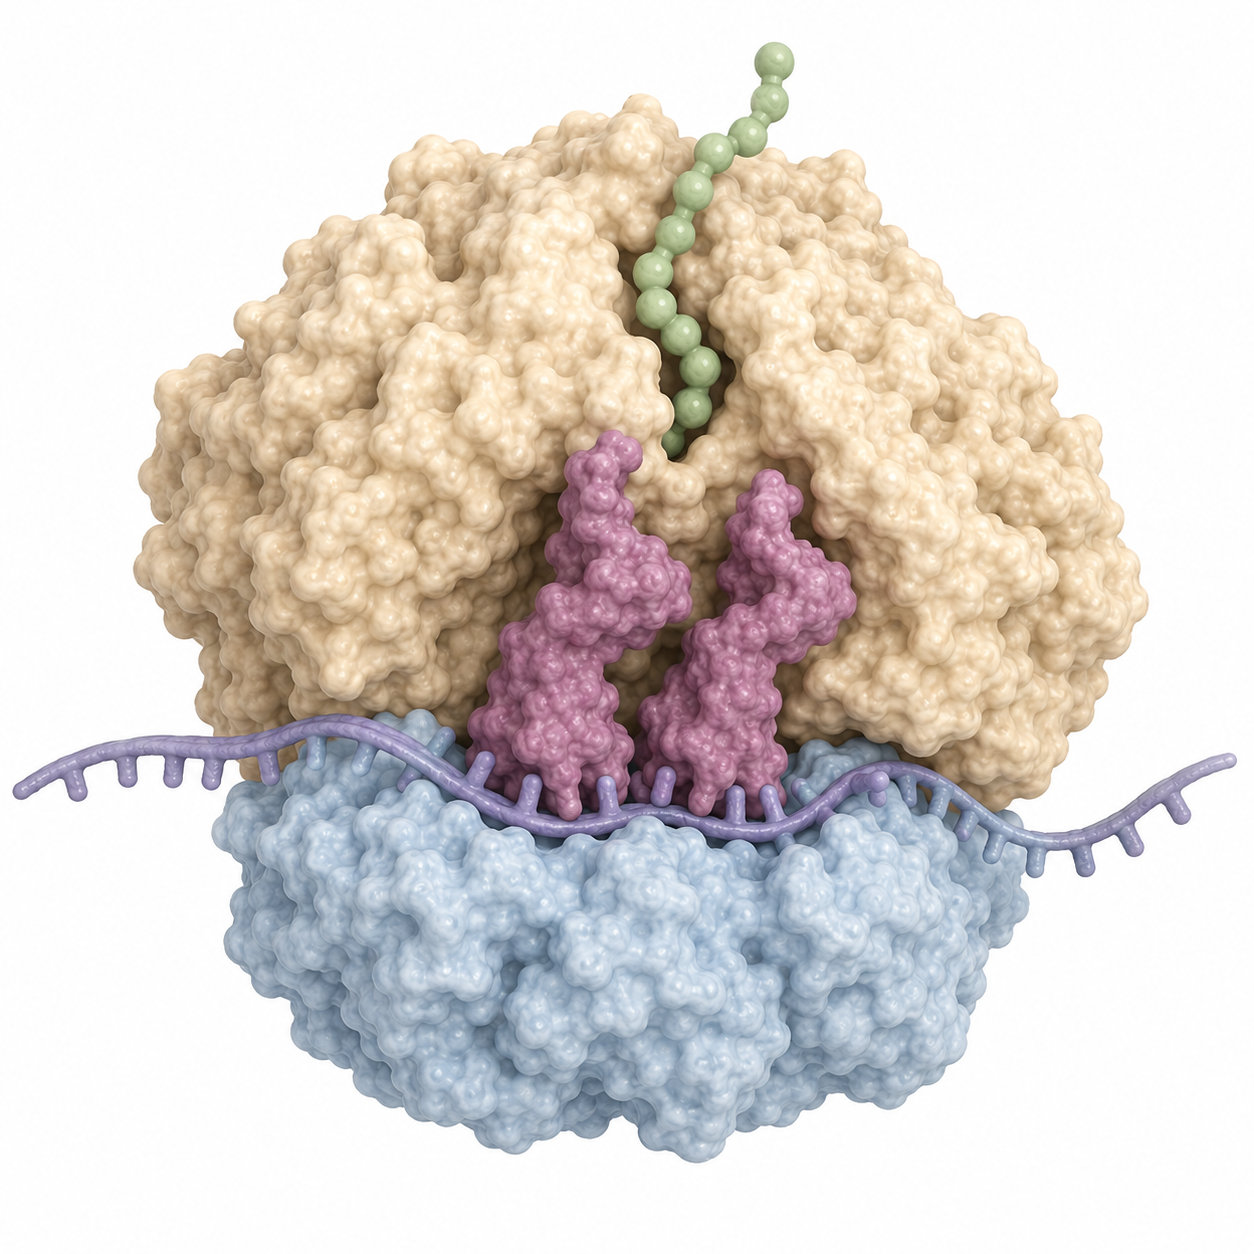
\includegraphics[width=0.46\linewidth]{images/book3/ai/fig-ribosome-3d.png}};
  \begin{scope}[x={(img.south east)}, y={(img.north west)},
      every node/.style={font=\small}]
    \draw[omDef, thick] (0.30,0.72) -- (0.30,1.08) node[above] {grote subeenheid: hier wordt de peptidebinding gemaakt};
    \draw[omDef, thick] (0.50,0.15) -- (0.50,-0.08) node[below] {kleine subeenheid: decodeert de boodschap};
    \draw[omDef, thick] (0.47,0.52) -- (-0.03,0.44) node[left, align=right] {tRNA's in de\\ P- en de A-plaats};
    \draw[omDef, thick] (0.92,0.36) -- (1.03,0.26) node[right] {mRNA};
    \draw[omDef, thick] (0.57,0.88) -- (1.03,0.90) node[right, align=left] {het polypeptide vertrekt\\ door de uitgangstunnel};
  \end{scope}
\end{tikzpicture}

{\small Het \omterm{def:b1:gene-expression:ribosome}{ribosoom}: twee subeenheden geklemd op de boodschapper, twee
\omterm{def:b1:gene-expression:trna}{transfer-RNA}'s in de spleet, en de groeiende keten die door een tunnel in de grote
subeenheid vertrekt.}
\end{omfigure}

\begin{proposition}[De cyclus van de verlenging]\label{prop:b1:gene-expression:elongation}
De \omterm{prop:b1:gene-expression:dogma}{translatie} begint wanneer de kleine subeenheid het startcodon vindt --- bij
bacteriën door een sequentie van \omterm{def:b1:nucleic-acids:rnas}{ribosomaal RNA} te paren met een plaats vlak vóór
de AUG, bij eukaryoten door de cap te binden en tot het eerste AUG te schuiven ---
en het start-tRNA (methionine) zich in de P-plaats nestelt; daarna sluit de grote
subeenheid zich erbij aan. Elke ronde \emph{verlenging} voegt één residu toe: een
geladen tRNA waarvan het \omterm{def:b1:gene-expression:trna}{anticodon} bij het \omterm{def:b1:gene-expression:code}{codon} in de A-plaats past wordt door een
verlengingsfactor afgeleverd en gecontroleerd (één GTP); het ribosomale \omterm{def:b1:nucleic-acids:chain}{RNA} van de
grote subeenheid draagt de groeiende keten van het tRNA in de P-plaats over op het
\omterm{def:b1:proteins:aminoacid}{aminozuur} van het tRNA in de A-plaats en vormt zo de \omterm{def:b1:proteins:peptide}{peptidebinding}; het \omterm{def:b1:gene-expression:ribosome}{ribosoom}
schuift één \omterm{def:b1:gene-expression:code}{codon} op (een tweede GTP), waarbij de tRNA's naar P en E verschuiven en
het lege vertrekt. Bij een stopcodon komt een \emph{afgiftefactor} de A-plaats
binnen en wordt de keten door \omterm{prop:b1:water-small-molecules:families}{hydrolyse} vrijgemaakt. Bacteriële \omterm{def:b1:gene-expression:ribosome}{ribosomen} voegen
vijftien tot twintig residuen per seconde toe, eukaryote twee tot vijf; meerdere
\omterm{def:b1:gene-expression:ribosome}{ribosomen} lezen één boodschap tegelijk en vormen een \emph{polysoom}.
\end{proposition}

\begin{omfigure}
\begin{tikzpicture}[font=\footnotesize, >=Stealth, line cap=round,
  rib/.style={draw, thick, rounded corners=8pt, fill=omDef!12, minimum width=30mm, minimum height=14mm},
  trna/.style={draw, thick, fill=omProp!30, minimum width=6mm, minimum height=9mm, inner sep=1pt, font=\scriptsize}]
  \foreach \i/\title in {0/{1. een geladen tRNA komt de A-plaats binnen}, 1/{2. peptidebinding: de keten gaat over op het tRNA in de A-plaats}, 2/{3. translocatie: het ribosoom schuift één codon op}} {
    \begin{scope}[xshift=\i*4.5cm]
      \node[rib] (r) at (0,0) {};
      \draw[very thick, omThm] (-2.0,-0.9) -- (2.0,-0.9);
      \node[font=\scriptsize] at (-0.45,-0.55) {P}; \node[font=\scriptsize] at (0.45,-0.55) {A};
      \node[anchor=north, align=center, font=\scriptsize, text width=40mm] at (0,-1.75) {\title};
    \end{scope}
  }
  % state 1: P holds chain, A receives new tRNA
  \node[trna] at (-0.45,0.05) {}; \draw[very thick, omExo!70!black] (-0.45,0.5) -- (-0.45,1.4); \foreach \y in {0.6,0.85,1.1,1.35} { \fill[omExo!70!black] (-0.45,\y) circle (0.09); }
  \node[trna] at (0.45,0.05) {}; \fill[omExo!70!black] (0.45,0.6) circle (0.09);
  \draw[->, thick, omProp!80!black] (1.6,1.3) -- (0.75,0.7); \node[font=\scriptsize, anchor=west] at (1.4,1.45) {GTP};
  % state 2: chain transferred
  \node[trna] at (4.05,0.05) {}; \node[trna] at (4.95,0.05) {}; \draw[very thick, omExo!70!black] (4.95,0.5) -- (4.95,1.65); \foreach \y in {0.6,0.85,1.1,1.35,1.6} { \fill[omExo!70!black] (4.95,\y) circle (0.09); }
  % state 3: translocated: chain on P, empty tRNA leaving at E, A free
  \node[trna, fill=gray!20] at (7.6,0.05) {}; \node[trna] at (8.55,0.05) {}; \draw[very thick, omExo!70!black] (8.55,0.5) -- (8.55,1.65); \foreach \y in {0.6,0.85,1.1,1.35,1.6} { \fill[omExo!70!black] (8.55,\y) circle (0.09); }
  \draw[->, thick, gray] (7.6,-0.4) -- (7.0,-1.0); \node[font=\scriptsize, gray, anchor=east] at (7.05,-0.4) {E};
  \draw[->, thick, omProp!80!black] (10.7,0.3) -- (10.7,-0.3); \node[font=\scriptsize, anchor=west] at (10.8,0.3) {GTP};
  \draw[->, thick, omThm] (9.4,-1.3) -- (10.4,-1.3) node[right, font=\scriptsize, omThm] {het mRNA schuift op};
\end{tikzpicture}

{\small Eén ronde verlenging. Een geladen tRNA wordt in de A-plaats toegelaten
wanneer zijn \omterm{def:b1:gene-expression:trna}{anticodon} past; het ribosomale \omterm{def:b1:nucleic-acids:chain}{RNA} verbindt de keten met zijn
\omterm{def:b1:proteins:aminoacid}{aminozuur}; het \omterm{def:b1:gene-expression:ribosome}{ribosoom} schuift één \omterm{def:b1:gene-expression:code}{codon} op, en het lege tRNA vertrekt. Twee GTP
per residu, plus de twee energierijke bindingen die het laden van het tRNA kost.}
\end{omfigure}

\begin{omfigure}
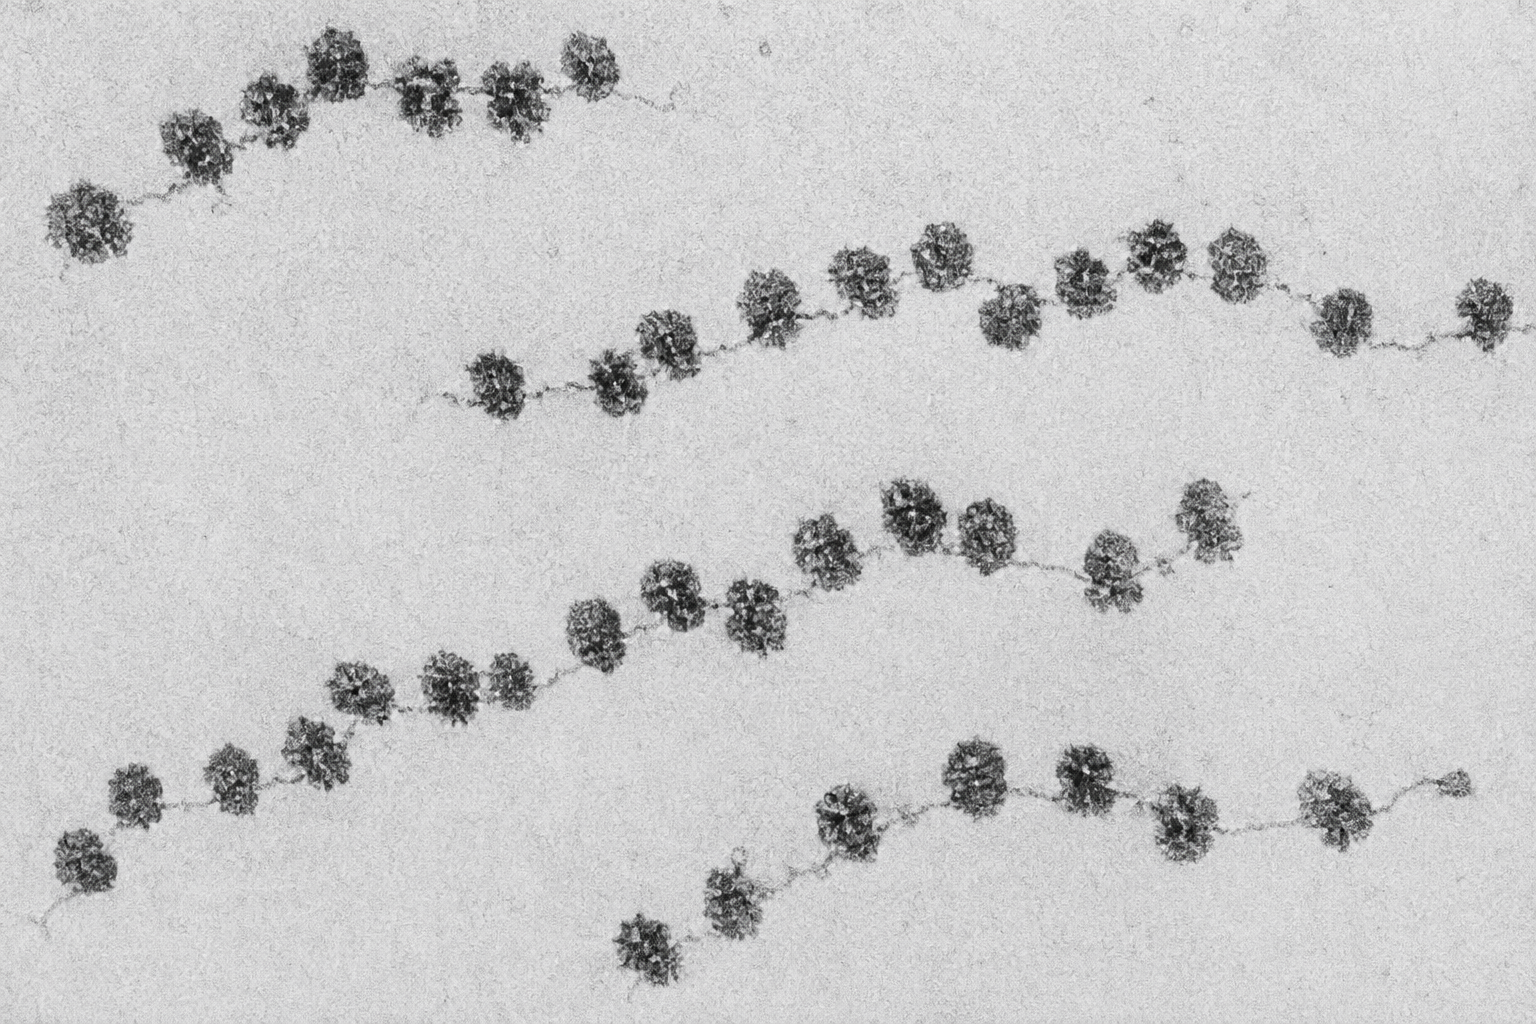
\includegraphics[width=0.5\linewidth]{images/book3/ai/b3-19-polysome-tem.png}

{\small Polysomen onder de \omterm{prop:b1:cell-unit-of-life:microscopes}{elektronenmicroscoop}: \omterm{def:b1:gene-expression:ribosome}{ribosomen} aaneengeregen langs een
boodschapper, die elk hun eigen kopie van het \omterm{def:b1:proteins:peptide}{eiwit} maken.}
\end{omfigure}

\begin{method}[De synthese van een eiwit becijferen]\label{met:b1:gene-expression:reckon}
\begin{enumerate}
  \item Lengte: een \omterm{def:b1:proteins:peptide}{eiwit} van $n$ residuen vraagt een coderende sequentie
        van $3n + 3$ \omterm{def:b1:nucleic-acids:nucleotide}{nucleotiden} (het stopcodon meegerekend), binnen een
        boodschapper die langer is door haar niet-vertaalde uiteinden en,
        in het \omterm{def:b1:genomes:gene}{gen}, door haar \omterm{def:b1:genomes:gene}{intronen}.
  \item Tijd: deel $n$ door de verlengingssnelheid (\qtyrange{15}{20}{} per
        seconde bij bacteriën, \qtyrange{2}{5}{} bij eukaryoten); de
        boodschap wordt om de \qtyrange{80}{100}{} \omterm{def:b1:nucleic-acids:nucleotide}{nucleotiden} door een
        \omterm{def:b1:gene-expression:ribosome}{ribosoom} gelezen, zodat de opbrengst per boodschap één keten per
        (afstand / snelheid) seconden is.
  \item Energie: vier energierijke fosfaatbindingen per residu (twee om het
        tRNA te laden, twee GTP op het \omterm{def:b1:gene-expression:ribosome}{ribosoom}), plus de \omterm{prop:b1:gene-expression:dogma}{transcriptie} van
        de boodschap tegen twee per \omterm{def:b1:nucleic-acids:nucleotide}{nucleotide}, verdeeld over alle ketens
        die die boodschap oplevert.
  \item Trouw: ongeveer één verkeerd \omterm{def:b1:proteins:aminoacid}{aminozuur} per $10^4$ \omterm{def:b1:gene-expression:code}{codons}; een \omterm{def:b1:proteins:peptide}{eiwit}
        van \qty{500}{} residuen is bij één kopie op twintig ergens fout
        --- draaglijk omdat \omterm{def:b1:proteins:peptide}{eiwitten} vervangbaar zijn en fouten niet worden
        geërfd.
\end{enumerate}
\end{method}

\section{Na de translatie}

\begin{proposition}[Wat er met een nieuw polypeptide gebeurt]\label{prop:b1:gene-expression:after}
\index{signaalpeptide}\index{posttranslationele modificatie}
De keten vouwt zich terwijl zij tevoorschijn komt, geholpen door \omterm{prop:b1:proteins:denaturation}{chaperonnes}
(\cref{ch:b1:proteins}). Haar bestemming staat in haar sequentie geschreven: een
\emph{\omterm{prop:b1:gene-expression:after}{signaalpeptide}} aan het N-uiteinde bindt een
\emph{signaalherkenningsdeeltje} dat de \omterm{prop:b1:gene-expression:dogma}{translatie} stillegt, het \omterm{def:b1:gene-expression:ribosome}{ribosoom} aan het
\omterm{def:b1:eukaryotic-cell:endomembrane}{endoplasmatisch reticulum} koppelt en de keten het lumen ervan in schuift
(\cref{ch:b1:eukaryotic-cell}); andere sequenties sturen \omterm{def:b1:proteins:peptide}{eiwitten} na de synthese
naar de \omterm{def:b1:eukaryotic-cell:mitochondrion}{mitochondriën}, de \omterm{def:b1:eukaryotic-cell:plastid}{chloroplasten}, de celkern of de \omterm{def:b1:eukaryotic-cell:peroxisome}{peroxisomen}; een \omterm{def:b1:proteins:peptide}{eiwit}
zonder signaal blijft in het \omterm{def:b1:eukaryotic-cell:organelle}{cytosol}. Veel \omterm{def:b1:proteins:peptide}{eiwitten} worden \emph{gewijzigd}: de
eerste methionine wordt verwijderd, in het ER en het \omterm{def:b1:eukaryotic-cell:endomembrane}{golgi-apparaat} komen er
suikers bij, kinasen en fosfatasen voegen fosfaten toe en halen ze weg, er worden
\omterm{def:b1:lipids:fattyacid}{lipiden} aangehecht, er worden stukken uitgeknipt (insuline wordt als één keten
gemaakt en in tweeën geknipt; zymogenen worden geknipt om ze te activeren). En elk
\omterm{def:b1:proteins:peptide}{eiwit} wordt uiteindelijk \emph{afgebroken}: gemerkt met het kleine \omterm{def:b1:proteins:peptide}{eiwit}
\emph{ubiquitine} en door het \emph{proteasoom} ontvouwen en verteerd, na een leven
van minuten (regeleiwitten) tot maanden (hemoglobine) --- zodat de aanwezige
\omterm{def:b1:proteins:peptide}{eiwitten} die zijn welke de \omterm{def:b1:cell-unit-of-life:cell}{cel} op dat moment maakt.
\end{proposition}

\begin{example}[De getallen van een cel]\label{ex:b1:gene-expression:numbers}
Een groeiende \emph{E. coli} bevat zo'n \num{20000} \omterm{def:b1:gene-expression:ribosome}{ribosomen}, die er elk twintig
residuen per seconde bij zetten: $\num{4e5}$ residuen per seconde, een miljoen
\omterm{def:b1:proteins:peptide}{eiwitten} van \qty{300}{} residuen in een uur --- haar eigen inhoud, en dat is wat
elk uur verdubbelen vraagt. De helft van haar energie gaat naar de eiwitsynthese.
Een levercel bevat tien miljoen \omterm{def:b1:gene-expression:ribosome}{ribosomen} en maakt \omterm{def:b1:proteins:peptide}{eiwitten} voor weken gebruik in
plaats van voor een deling; een plasmacel, die antistof afscheidt, zet er vrijwel
alle in voor één \omterm{def:b1:proteins:peptide}{eiwit} en stort tweeduizend moleculen per seconde uit.
\end{example}

\section{Opgaven}

\begin{exercise}[$\star$]\label{exo:b1:gene-expression:1}
Geef het \omterm{def:b1:nucleic-acids:chain}{RNA} dat van de matrijsstreng $3'$-TACGGATTC-$5'$ wordt overgeschreven, en
de coderende streng.
\end{exercise}

\begin{exercise}[$\star$]\label{exo:b1:gene-expression:2}
Noem de drie wijzigingen die een eukaryoot primair transcript ondergaat voordat het
de celkern verlaat.
\end{exercise}

\begin{exercise}[$\star$]\label{exo:b1:gene-expression:3}
Vertaal met de codetabel $5'$-AUGCCGAAAGUUUGA-$3'$.
\end{exercise}

\begin{exercise}[$\star$]\label{exo:b1:gene-expression:4}
Noem de drie tRNA-plaatsen van het \omterm{def:b1:gene-expression:ribosome}{ribosoom} en wat er in elk gebeurt.
\end{exercise}

\begin{exercise}[$\star\star$]\label{exo:b1:gene-expression:5}
Een boodschapper van \qty{2400}{} \omterm{def:b1:nucleic-acids:nucleotide}{nucleotiden} heeft \qty{150}{} \omterm{def:b1:nucleic-acids:nucleotide}{nucleotiden}
niet-vertaald $5'$-gebied en \qty{450}{} niet-vertaald $3'$-gebied plus poly-A.
Hoeveel residuen telt het \omterm{def:b1:proteins:peptide}{eiwit}? Hoe lang doet één \omterm{def:b1:gene-expression:ribosome}{ribosoom} erover bij vier
residuen per seconde, en hoeveel \omterm{def:b1:gene-expression:ribosome}{ribosomen} kunnen de boodschap tegelijk lezen bij
één per \qty{90}{} \omterm{def:b1:nucleic-acids:nucleotide}{nucleotiden}?
\end{exercise}

\begin{exercise}[$\star\star$]\label{exo:b1:gene-expression:6}
Leg uit waarom drie invoegingen het \omterm{def:b1:gene-expression:code}{leesraam} van een \omterm{def:b1:genomes:gene}{gen} herstellen en één of twee
niet, en hoe het \omterm{def:b1:proteins:peptide}{eiwit} uit de drievoudige invoeging eruitziet.
\end{exercise}

\begin{exercise}[$\star\star$]\label{exo:b1:gene-expression:7}
Een mutatie verandert het \omterm{def:b1:gene-expression:code}{codon} CAG in UAG midden in een \omterm{def:b1:genomes:gene}{gen} van \qty{300}{}
\omterm{def:b1:gene-expression:code}{codons}; een andere verandert CAG in CAA; een derde verandert het in CGG. Geef het
effect van elk op het \omterm{def:b1:proteins:peptide}{eiwit}.
\end{exercise}

\begin{exercise}[$\star\star$]\label{exo:b1:gene-expression:8}
Leg uit waarom de trouw van de \omterm{prop:b1:gene-expression:dogma}{translatie} op de \omterm{def:b1:gene-expression:trna}{aminoacyl-tRNA-synthetasen} berust
en niet op het \omterm{def:b1:gene-expression:ribosome}{ribosoom}, en beschrijf een proef die dat aantoonde (een cysteïne die
aan haar tRNA vastzit wordt chemisch in alanine omgezet; waar komt het alanine
terecht?).
\end{exercise}

\begin{exercise}[$\star\star$]\label{exo:b1:gene-expression:9}
Bereken de energiekosten, in energierijke bindingen, van een \omterm{def:b1:proteins:peptide}{eiwit} van \qty{400}{}
residuen, en het deel daarvan dat op het \omterm{def:b1:gene-expression:ribosome}{ribosoom} wordt uitgegeven.
\end{exercise}

\begin{exercise}[$\star\star\star$]\label{exo:b1:gene-expression:10}
Bij bacteriën beginnen \omterm{def:b1:gene-expression:ribosome}{ribosomen} een boodschap te vertalen terwijl die nog wordt
overgeschreven; bij eukaryoten kan dat niet. Leg uit waarom (twee redenen), en wat
dit verschil bij eukaryoten mogelijk maakt.
\end{exercise}

\begin{exercise}[$\star\star\star$]\label{exo:b1:gene-expression:11}
Een \omterm{def:b1:genomes:gene}{gen} met vijf \omterm{def:b1:genomes:gene}{exonen} kan zo worden gespliced dat \omterm{def:b1:genomes:gene}{exon} 3 (\qty{90}{} \omterm{def:b1:nucleic-acids:nucleotide}{nucleotiden})
en \omterm{def:b1:genomes:gene}{exon} 4 (\qty{100}{} \omterm{def:b1:nucleic-acids:nucleotide}{nucleotiden}) worden meegenomen of overgeslagen. Noem de
mogelijke boodschappers en zeg welke het \omterm{def:b1:gene-expression:code}{leesraam} van \omterm{def:b1:genomes:gene}{exon} 5 behouden. Wat laat dat
zien over alternatieve \omterm{prop:b1:gene-expression:processing}{splicing}?
\end{exercise}

\begin{exercise}[$\star\star\star$]\label{exo:b1:gene-expression:12}
``De code is een bevroren toeval: willekeurig, maar te duur om te veranderen.''
Bespreek dat in een korte alinea: wat er in de code willekeurig lijkt, wat er
geoptimaliseerd lijkt (de derde plaats, verwante \omterm{def:b1:gene-expression:code}{codons} voor verwante \omterm{def:b1:proteins:aminoacid}{aminozuren}),
en waarom een mutatie die de specificiteit van een synthetase verandert vrijwel
altijd dodelijk is.
\end{exercise}

\section{Vraagstuk: van een gen naar een eiwit}

\begin{problem}[{Weekendvraagstuk --- een gen van dertig kilobasen gevolgd tot een
eiwit van vijfhonderd residuen: de transcriptie geklokt, de splicing gewogen, de
ribosomen geteld, de energie en de fouten becijferd, eindigend op de kosten van
één eiwit in ATP}]
\label{pb:b1:gene-expression:1}
Een menselijk \omterm{def:b1:genomes:gene}{gen} beslaat \qty{30}{kb} met acht \omterm{def:b1:genomes:gene}{exonen} die samen \qty{2000}{}
\omterm{def:b1:nucleic-acids:nucleotide}{nucleotiden} rijpe boodschapper vormen, waarvan er \qty{1503}{} coderen (500
residuen plus de stop). Polymerase II schrijft \qty{30}{} \omterm{def:b1:nucleic-acids:nucleotide}{nucleotiden} per seconde
over; \omterm{def:b1:gene-expression:ribosome}{ribosomen} verlengen met \qty{4}{} residuen per seconde en houden onderling
één per \qty{80}{} \omterm{def:b1:nucleic-acids:nucleotide}{nucleotiden} afstand; de halveringstijd van de boodschapper is
\qty{2}{h}. Kosten: twee energierijke bindingen per overgeschreven \omterm{def:b1:nucleic-acids:nucleotide}{nucleotide}, vier
per vertaald residu; neem één energierijke binding als één \omterm{def:b1:water-small-molecules:atp}{ATP}. Foutfrequenties:
$10^{-5}$ per overgeschreven \omterm{def:b1:nucleic-acids:nucleotide}{nucleotide}, $10^{-4}$ per vertaald \omterm{def:b1:gene-expression:code}{codon}.

\medskip
\noindent\textbf{Deel I --- \omterm{prop:b1:gene-expression:dogma}{Transcriptie} en \omterm{prop:b1:gene-expression:processing}{splicing}.}
\begin{enumerate}
  \item Hoe lang doet één polymerase erover om het \omterm{def:b1:genomes:gene}{gen} over te schrijven?
  \item Welk deel van het primaire transcript wordt er door de \omterm{prop:b1:gene-expression:processing}{splicing}
        verwijderd?
  \item Hoeveel \omterm{def:b1:nucleic-acids:nucleotide}{nucleotiden} worden er overgeschreven per \omterm{def:b1:nucleic-acids:nucleotide}{nucleotide} rijpe
        boodschapper?
  \item Bereken het \omterm{def:b1:water-small-molecules:atp}{ATP} dat aan het overschrijven van één primair
        transcript wordt besteed.
  \item Als er elke \qty{10}{s} een polymerase begint, hoeveel polymerasen
        zitten er dan tegelijk op het \omterm{def:b1:genomes:gene}{gen}, en hoeveel boodschappers levert
        het \omterm{def:b1:genomes:gene}{gen} per uur op?
  \item Bereken het aantal \omterm{def:b1:genomes:gene}{intronen} en hun gemiddelde lengte.
  \item Het spliceosoom verwijdert elk \omterm{def:b1:genomes:gene}{intron} in ongeveer een minuut,
        parallel. Bepaalt de \omterm{prop:b1:gene-expression:processing}{splicing} of de \omterm{prop:b1:gene-expression:dogma}{transcriptie} de tijd van \omterm{def:b1:genomes:gene}{gen}
        tot boodschapper?
  \item Bereken de fysieke lengte van het \omterm{def:b1:genomes:gene}{gen} en van de rijpe boodschapper
        (\qty{0.34}{nm} per \omterm{def:b1:nucleic-acids:nucleotide}{nucleotide}).
\end{enumerate}

\medskip
\noindent\textbf{Deel II --- \omterm{prop:b1:gene-expression:dogma}{Translatie}.}
\begin{enumerate}[resume]
  \item Hoe lang doet één \omterm{def:b1:gene-expression:ribosome}{ribosoom} erover om het \omterm{def:b1:proteins:peptide}{eiwit} te vertalen?
  \item Hoeveel \omterm{def:b1:gene-expression:ribosome}{ribosomen} lezen één boodschapper tegelijk?
  \item Hoeveel eiwitmoleculen levert één boodschapper per uur op?
  \item Hoeveel levert zij er over haar halveringstijd van \qty{2}{h} in
        totaal op (een boodschap met halveringstijd $t_{1/2}$ levert
        gemiddeld $t_{1/2}/\ln 2$ uur volle productie)?
  \item Bereken het \omterm{def:b1:water-small-molecules:atp}{ATP} dat aan het vertalen van één \omterm{def:b1:proteins:peptide}{eiwit} wordt besteed.
  \item Bereken het \omterm{def:b1:water-small-molecules:atp}{ATP} dat per \omterm{def:b1:proteins:peptide}{eiwit} aan de \omterm{prop:b1:gene-expression:dogma}{transcriptie} wordt besteed,
        door de kosten van het transcript over de \omterm{def:b1:proteins:peptide}{eiwitten} uit vraag 12 te
        verdelen.
  \item Bereken de totale kosten van één \omterm{def:b1:proteins:peptide}{eiwit} en het deel dat aan de
        \omterm{prop:b1:gene-expression:dogma}{translatie} is toe te schrijven.
\end{enumerate}

\medskip
\noindent\textbf{Deel III --- Fouten.}
\begin{enumerate}[resume]
  \item Bereken de kans dat een bepaalde boodschapper ten minste één
        transcriptiefout draagt in haar \qty{1503}{} coderende \omterm{def:b1:nucleic-acids:nucleotide}{nucleotiden}.
  \item Bereken de kans dat een bepaald eiwitmolecuul ten minste één
        translatiefout draagt.
  \item Ongeveer een kwart van de veranderingen van een \omterm{def:b1:nucleic-acids:nucleotide}{nucleotide} is stil
        en een derde van de vervangingen van een \omterm{def:b1:proteins:aminoacid}{aminozuur} is onschadelijk.
        Welk deel van de gemaakte eiwitmoleculen is defect?
  \item Een defecte boodschapper levert twee uur lang defecte \omterm{def:b1:proteins:peptide}{eiwitten} op;
        een defect \omterm{def:b1:proteins:peptide}{eiwit} is één molecuul. Leg uit waarom de \omterm{def:b1:cell-unit-of-life:cell}{cel} zich een
        translatiefoutfrequentie kan veroorloven die tien keer die van de
        \omterm{prop:b1:gene-expression:dogma}{transcriptie} is, en beide ver boven die van de replicatie.
\end{enumerate}

\medskip
\noindent\textbf{Deel IV --- De begroting van de \omterm{def:b1:cell-unit-of-life:cell}{cel}.}
De \omterm{def:b1:cell-unit-of-life:cell}{cel} maakt per uur \num{3000} kopieën van dit \omterm{def:b1:proteins:peptide}{eiwit}, en in totaal \num{3e9}
residuen \omterm{def:b1:proteins:peptide}{eiwit} per dag.
\begin{enumerate}[resume]
  \item Hoeveel boodschappers van dit \omterm{def:b1:genomes:gene}{gen} moeten er tegelijk aanwezig zijn
        (elk met de opbrengst uit vraag 11)?
  \item Hoeveel \omterm{def:b1:gene-expression:ribosome}{ribosomen} zijn er met dit \omterm{def:b1:proteins:peptide}{eiwit} bezig?
  \item Bereken het \omterm{def:b1:water-small-molecules:atp}{ATP} dat de \omterm{def:b1:cell-unit-of-life:cell}{cel} per dag aan al haar eiwitsynthese
        besteedt (vier per residu) en, bij \qty{50}{kJ/mol}, het vermogen
        in watt voor een \omterm{def:b1:cell-unit-of-life:cell}{cel} van \qty{2000}{\micro m^3}.
  \item Vergelijk dat met het totale vermogen van de \omterm{def:b1:cell-unit-of-life:cell}{cel} als zij
        \qty{1e9}{} \omterm{def:b1:water-small-molecules:atp}{ATP} per seconde verbruikt.
  \item Een geneesmiddel blokkeert het spliceosoom. Voorspel het effect
        ervan op dit \omterm{def:b1:proteins:peptide}{eiwit} en op een bacterieel \omterm{def:b1:proteins:peptide}{eiwit}.
  \item Geef het resultaat: de ATP-kosten van één molecuul van het \omterm{def:b1:proteins:peptide}{eiwit},
        verdeeld over \omterm{prop:b1:gene-expression:dogma}{translatie} en \omterm{prop:b1:gene-expression:dogma}{transcriptie}, en de tijd van het begin
        van de \omterm{prop:b1:gene-expression:dogma}{transcriptie} tot het eerste voltooide \omterm{def:b1:proteins:peptide}{eiwit}.
\end{enumerate}
\end{problem}
